% ----------------------------------------------------------
\chapter{Revisão Bibliográfica}\label{cap:revisao}
% ----------------------------------------------------------

\section{A Logística de Produtos Perecíveis no Agronegócio}

A logística de produtos perecíveis, particularmente no setor de hortifrúti, possui uma complexidade elevada devido à natureza biológica dos produtos. Diferente de produtos industrializados, os perecíveis possuem uma vida útil curta e continuam seus processos metabólicos mesmo após a colheita, o que exige uma gestão da cadeia de suprimentos ágil e eficiente para evitar a perda comercial.

\subsection{O Panorama do Desperdício}

O desperdício de alimentos é um dos maiores desafios logísticos que o mundo enfrenta atualmente. Segundo a Organização das Nações Unidas para a Alimentação e a Agricultura \cite{FAO2011}, cerca de um terço de todos os alimentos produzidos no mundo para consumo humano é perdido ou desperdiçado anualmente. No contexto brasileiro, essa realidade é agravada por gargalos infraestruturais e processos de manuseio inadequados.

% ----------------------------------------------------------
\section{O Tomate-Cereja e sua Classificação Comercial}
% ----------------------------------------------------------

No Brasil, a classificação comercial do tomate segue as normas do Programa Brasileiro para a Modernização da Horticultura (PBMH) \cite{ceagesp2003}, que avaliam atributos externos observáveis divididos em quatro critérios: formato, tamanho, coloração e tolerância a defeitos. Os defeitos são classificados em leves ou graves. Os graves possuem uma tolerância menor por afetarem o consumo ou a conservação do fruto. Por serem parâmetros tratados de forma independente na norma, justifica-se o uso de técnicas específicas para cada um desses parâmetros em um sistema automático.

\subsection{Estados de maturação}

A maturação do tomate manifesta-se principalmente pela mudança de cor da casca, do verde para o vermelho, resultado da degradação da clorofila e da síntese de carotenoides, em especial o licopeno. O padrão de classificação do Departamento de Agricultura dos Estados Unidos (USDA) \cite{usda1991} define seis estados de maturação pela fração da superfície que mudou de cor, conforme ilustrado na Figura~\ref{fig:maturacao_usda}.

\begin{figure}[H]
    \centering
    \caption{Estádios de maturação do tomate segundo o padrão do USDA.}
    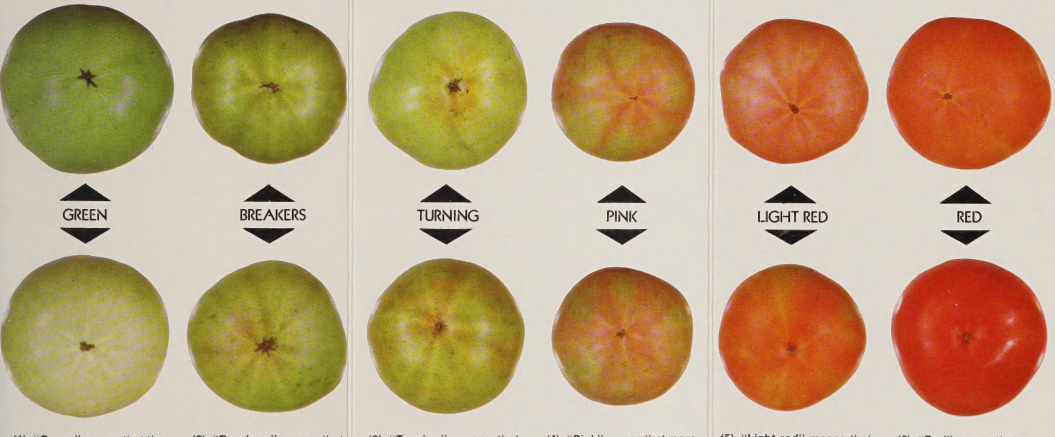
\includegraphics[width=0.85\textwidth]{images/imagem_usda1991.png}
    \label{fig:maturacao_usda}
    \legend{Fonte: \textcite{usda1991}.}
\end{figure}

Dois critérios desse padrão são determinantes para sistemas automatizados de classificação. Primeiramente a avaliação baseada na proporção de área atingida, em vez da média global de cor, e a transição de cor progressiva, na qual os estados iniciais admitem tonalidades amarelas, enquanto os finais exigem de forma predominante tons avermelhados e vermelhos. Para simplificar a rotulagem das amostras neste trabalho, os seis estados originais do USDA foram agrupados em três classes, sendo elas imaturo, intermediário e maduro. Embora \textcite{hou2024} também empreguem a fração de área vermelha como métrica, os autores adotam limiares de 80\% e 90\%, restringindo a classificação a frutos já avermelhados destinados ao consumo \textit{in natura}.

\subsection{Defeitos externos e calibre}

Os defeitos externos do tomate incluem rachaduras, podridões e mofos, danos mecânicos e manchas. Diferentemente da cor, os defeitos são padrões locais de textura e forma, de aparência muito variável, o que dificulta descrevê-los por regras explícitas \cite{dacosta2020}. Já o tamanho é uma grandeza geométrica. Para os tomates de mesa dos grupos redondo e oblongo, a classe é definida pelo maior diâmetro transversal \cite{ceagesp2003}; o tomate-cereja não segue esse mesmo critério de diâmetro, e por isso este trabalho mede o tamanho dos frutos, mas não os separa em classes de calibre. Em qualquer caso, medir o tamanho a partir da imagem exige converter medidas em pixels para milímetros.

% ----------------------------------------------------------
\section{Visão Computacional}
% ----------------------------------------------------------

Visão computacional é o conjunto de técnicas que extrai informações úteis de imagens digitais. Na inspeção de alimentos, ela permite realizar medições sem contato, não destrutivas e consistentes, substituindo aos poucos a inspeção visual humana, que é lenta, cansativa e subjetiva \cite{brosnan2004,cubero2011}. \textcite{chen2002} descrevem que um sistema de visão computacional para aplicações agrícolas é formado pela combinação de iluminação, câmera, placa de aquisição e software, em que o processamento consiste no realce da imagem, extração de características e classificação.

\subsection{Cor digital e balanço de branco}

Uma câmera digital registra, em cada pixel $(x,y)$, a resposta de três sensores, onde cada sensor representa um canal de cor: vermelho, verde e azul. No modelo físico de formação da imagem com iluminação uniforme, a resposta \(c_i(x,y)\) de cada canal \(i \in \{r, g, b\}\) depende do fator geométrico de sombreamento \(G(x,y)\), da reflectância espectral do objeto \(R_i(x,y)\) e da intensidade da fonte de luz \(L_{i}\) \cite{ebner2007}. Como uma mesma fruta fotografada sob diferentes condições de luz produz valores \acs{RGB} diferentes, torna-se necessário compensar o efeito da iluminação para que a cor medida represente fielmente o objeto \cite{ebner2007}.

Para transformar uma imagem capturada sob um iluminante \(L\) para um iluminante de referência \(L'\), o modelo diagonal de adaptação de von Kries aplica um fator de escala independente a cada canal de cor:
\[
\begin{bmatrix}
c_{r}^{\prime} \\
c_{g}^{\prime} \\
c_{b}^{\prime}
\end{bmatrix}
=
\begin{bmatrix}
k_{r} & 0 & 0 \\
0 & k_{g} & 0 \\
0 & 0 & k_{b}
\end{bmatrix}
\begin{bmatrix}
c_{r} \\
c_{g} \\
c_{b}
\end{bmatrix},
\qquad k_{i}=\frac{L_{i}^{\prime}}{L_{i}}
\]
Como o iluminante real \(L_{i}\) geralmente é desconhecido, a compensação exige obter uma estimativa \(\tilde{L}_i \approx L_i\) que permita normalizar cada canal da imagem e recuperar a reflectância do objeto (com o fator de sombreamento):
\[
\frac{c_{i}(x,y)}{\tilde{L}_{i}} = \frac{G(x,y)\,R_{i}(x,y)\,L_{i}}{\tilde{L}_{i}} \approx G(x,y)\,R_{i}(x,y)
\]
Em sistemas com iluminação controlada, como bancadas de inspeção visual, essa estimativa é obtida diretamente pela medição de uma superfície de referência branca sob a mesma fonte de luz \cite{ebner2007}. A partir dos valores registrados nessa referência, calcula-se um ganho por canal \(k_{i}\) para equilibrar as respostas e ajustar o branco medido a um valor neutro, corrigindo o balanço de branco de toda a cena.

\subsection{Segmentação e morfologia matemática}

A segmentação divide a imagem em regiões distintas, separando os pixels do objeto de interesse dos pixels do fundo \cite{gonzalez2010}. Quando o objeto apresenta alto contraste em relação a um fundo uniforme, a limiarização global define uma máscara binária a partir de um limiar de intensidade \(T\):
\[
B(x,y) =
\begin{cases}
1, & \text{se } f(x,y) > T, \\
0, & \text{caso contrário,}
\end{cases}
\]
em que \(f(x,y)\) representa a imagem em tons de cinza que será segmentada.

O método de \textcite{otsu1979} encontra o limiar ótimo \(T^{*}\) automaticamente a partir do histograma normalizado de \(L\) níveis de intensidade, com probabilidades \(p_k = n_k / N\) para \(k \in \{0, 1, \dots, L-1\}\), onde \(n_{k}\) é o número de pixels no nível \(k\) e \(N\) é o total de pixels. Para um limiar candidato \(t\), os pixels são divididos em duas classes, \(C_0\) (intensidades até \(t\)) e \(C_1\) (intensidades acima de \(t\)), com probabilidades acumuladas \(\omega_0(t)\) e \(\omega_1(t)\) e médias \(\mu_0(t)\) e \(\mu_1(t)\). O limiar ótimo maximiza a variância entre classes \(\sigma_B^2(t)\):
\[
\sigma_{B}^{2}(t) = \omega_{0}(t)\omega_{1}(t)\left[\mu_{1}(t)-\mu_{0}(t)\right]^{2},
\qquad T^{*} = \arg\max_{0 \le t < L-1} \sigma_{B}^{2}(t).
\]
Esse critério estatístico torna a escolha do limiar menos sensível a pequenas variações de iluminação entre as capturas.

Porém, na prática, a aplicação direta da limiarização é bastante afetada por ruídos de captura e reflexos. A filtragem passa-baixa prévia reduz o ruído antes do cálculo do limiar, enquanto operações de morfologia matemática refinam a máscara binária \(B\). As mais usadas são a abertura morfológica, que suaviza contornos e elimina pequenos ruídos isolados, e o fechamento morfológico, que une regiões fragmentadas e preenche falhas internas.

\subsection{Calibração geométrica e medição de tamanho}

Para medir em milímetros, é preciso conhecer a relação entre pixels e unidades reais no plano do objeto. A calibração de câmera usando um padrão plano de geometria conhecida, como um tabuleiro de xadrez, é um método clássico \cite{zhang2000}; os cantos do tabuleiro podem ser detectados com precisão subpixel e alta confiabilidade pelo detector de \textcite{duda2018}, disponível na biblioteca OpenCV. Como a lente e a perspectiva fazem a escala variar ao longo da imagem, uma alternativa simples à modelagem completa da câmera é estimar a escala localmente, em diferentes regiões da área de trabalho, a partir das distâncias conhecidas entre cantos vizinhos do tabuleiro. Essa simplificação tem uma limitação própria do modelo de câmera pinhole \cite{zhang2000}: a escala é válida para o plano do tabuleiro, enquanto o contorno visível do fruto está alguns milímetros acima dele, mais próximo da câmera, o que gera uma pequena superestimativa na medida.

\begin{figure}[H]
    \centering
    \caption{Exemplos de vistas de um padrão planar em diferentes orientações para calibração de câmera.}
    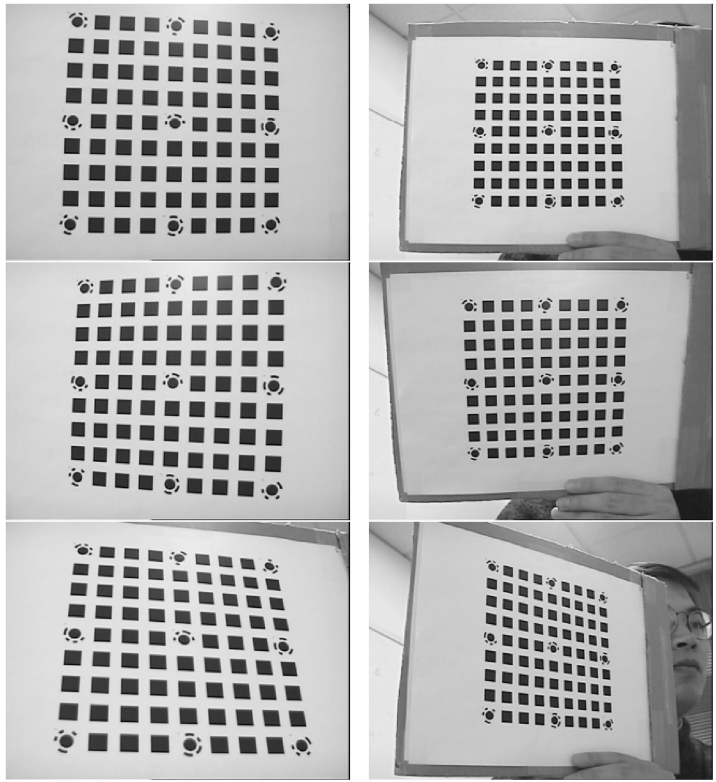
\includegraphics[width=0.85\textwidth]{images/imagem_zhang2000.png}
    \label{fig:calibracao_zhang2000}
    \legend{Fonte: Adaptado de \textcite{zhang2000}.}
\end{figure}

% ----------------------------------------------------------
\section{Classificação de Cor por Tabela de Consulta}
% ----------------------------------------------------------

Classificar cada pixel de uma imagem usando um modelo estatístico exige muito processamento para rodar em tempo real. Para resolver esse problema, utiliza-se uma tabela de consulta (\textit{lookup table}, LUT). Como uma imagem de 8 bits por canal possui \(256^3 \approx 16{,}7\) milhões de cores possíveis, o classificador pode ser avaliado uma única vez para todas elas, armazenando o resultado em uma tabela indexada pela própria cor. Assim, durante a execução, classificar um pixel passa a ser apenas uma leitura direta na memória.

\subsection{Agrupamento de cores com \textit{k-means}}

Rotular manualmente milhares de pixels para análise de cor é inviável na prática. Por isso, o algoritmo \textit{k-means} \cite{macqueen1967} resolve esse problema dividindo um conjunto de vetores de características \(\mathbf{x}_n \in \mathbb{R}^d\) (\(n = 1, \dots, N\)), onde cada \(\mathbf{x}_{n}\) representa os atributos de cor de um pixel, em \(k\) grupos distintos \(S_1, S_2, \dots, S_k\). O algoritmo busca minimizar a soma das distâncias ao quadrado entre cada ponto e o centro do seu grupo:
\[
J = \sum_{j=1}^{k} \sum_{\mathbf{x}_{n} \in S_{j}} \left\| \mathbf{x}_{n} - \boldsymbol{\mu}_{j} \right\|_{2}^{2},
\]
em que \(\boldsymbol{\mu}_{j}\) é o centroide do grupo \(S_{j}\) e \(\|\cdot\|_2\) representa a norma euclidiana. Na prática, o procedimento alterna entre atribuir cada pixel ao centroide mais próximo e recalcular a posição desses centroides até atingir a convergência.

Como a otimização de \(J\) é não convexa, o resultado final depende dos centros iniciais e pode convergir para mínimos locais. A inicialização \textit{k-means++} \cite{arthur2007} reduz esse problema escolhendo centros iniciais mais distantes entre si, de modo que pontos longe dos centros já selecionados tenham maior probabilidade de serem sorteados, tornando o agrupamento mais estável e consistente.

\subsection{Perceptron multicamadas}

O perceptron multicamadas (MLP) é uma rede neural com uma ou mais camadas ocultas de neurônios com função de ativação não linear, treinada pelo algoritmo de retropropagação do erro \cite{rumelhart1986}. Com neurônios ocultos suficientes, uma MLP consegue aproximar qualquer função contínua \cite{hornik1989}. Isso permite que ela aprenda fronteiras de decisão não lineares entre as classes de cor, ajustadas aos pixels rotulados, sem ficar presa às divisões rígidas que aconteceriam se cada cor fosse ligada apenas ao centro de grupo mais próximo. Os rótulos de treino vêm do agrupamento, mas a MLP permite unir vários grupos em uma mesma classe com uma fronteira contínua e ainda incluir a classe do fundo, que não entra na etapa de agrupamento.

A combinação entre MLP e LUT une a flexibilidade da rede com o baixo custo computacional da tabela. A principal limitação vem diretamente dos dados de treino: a tabela só é confiável para as cores observadas nas condições de iluminação da calibração, fazendo com que cores muito diferentes das vistas no treino recebam uma classificação estimada por extrapolação da rede.

% ----------------------------------------------------------
\section{Aprendizado Profundo e Redes Neurais Convolucionais}
% ----------------------------------------------------------

Defeitos como podridão, rachaduras e danos mecânicos são difíceis de descrever pela cor de pixels isolados: dependem de textura, forma e contexto espacial. O aprendizado profundo contorna essa dificuldade aprendendo as próprias características a partir dos dados, em múltiplos níveis de abstração \cite{lecun2015,goodfellow2016}. \textcite{kamilaris2018}, em uma revisão de 40 trabalhos de aplicação agrícola, observam que o aprendizado profundo superou, na maior parte deles, as técnicas de processamento de imagem comumente usadas.

\subsection{Redes neurais convolucionais}

As redes neurais convolucionais (\textit{convolutional neural networks}, CNN) são redes especializadas em imagens. Em vez de conectar cada pixel a cada neurônio, aplicam pequenos filtros que percorrem a imagem (convolução), compartilhando pesos e preservando a estrutura espacial \cite{lecun2015,goodfellow2016}. \textcite{zeiler2014} mostraram, ao visualizar redes treinadas, que as primeiras camadas respondem a bordas e manchas de cor e as seguintes a texturas e partes de objetos. Uma camada final, totalmente conectada, produz a pontuação de cada classe, convertida em probabilidades pela função \textit{softmax}. O trabalho de \textcite{krizhevsky2012} na competição ImageNet consolidou as CNN como o estado da arte em classificação de imagens.

Redes mais profundas, contudo, eram difíceis de otimizar: a partir de certa profundidade, o próprio erro de treinamento aumentava com o acréscimo de camadas. As redes residuais (ResNet) de \textcite{he2016} contornaram esse problema com conexões de atalho, que somam a entrada de um bloco à sua saída; assim, cada bloco aprende apenas uma correção residual em relação à identidade, o que facilita a otimização de redes profundas. Na ResNet, cada convolução é seguida de normalização em lote (\textit{batch normalization}) \cite{ioffe2015}, que estabiliza e acelera o treinamento. A ResNet-18, versão com 18 camadas \cite{he2016} e cerca de 11,7 milhões de parâmetros na implementação da biblioteca torchvision, é a menor da família, o que a torna adequada a conjuntos de dados pequenos e à execução em computadores sem placa de vídeo dedicada.

\subsection{Transferência de aprendizado}

Treinar uma CNN do zero exige grandes conjuntos de dados; com poucas centenas de imagens, a rede tende a memorizar os exemplos (sobreajuste). A transferência de aprendizado aproveita uma rede previamente treinada em um conjunto grande e genérico, como o ImageNet \cite{deng2009}, e a adapta à nova tarefa \cite{pan2010}. \textcite{yosinski2014} mostraram que as primeiras camadas de uma CNN aprendem características gerais, úteis para quase qualquer imagem, enquanto as últimas são específicas da tarefa original. Na prática, substitui-se a camada final por uma com o número de classes desejado e ajusta-se a rede inteira com taxa de aprendizado pequena (\textit{fine-tuning}), para não destruir as características já aprendidas. Em tomates, \textcite{dacosta2020} compararam o uso de ResNets pré-treinadas apenas como extratoras de características com o ajuste fino da rede na detecção de defeitos externos, em um conjunto de 43.843 imagens, e relatam vantagem do ajuste fino quando há dados suficientes.

\subsection{Aumento de dados e otimização}

O aumento de dados (\textit{data augmentation}) gera variações plausíveis das imagens de treino, como rotações, espelhamentos, recortes e pequenas alterações de brilho, ampliando artificialmente o conjunto e reduzindo o sobreajuste \cite{shorten2019}. As transformações devem respeitar a física do problema: um fruto pode aparecer em qualquer orientação, então rotações livres são válidas; já alterações fortes de cor seriam inadequadas para um sistema que usa a cor como critério e opera com iluminação calibrada.

O treinamento ajusta os pesos para minimizar uma função de perda, tipicamente a entropia cruzada, por descida de gradiente estocástica. O otimizador Adam \cite{kingma2015} adapta a taxa de aprendizado de cada peso a partir de estimativas dos momentos do gradiente; a variante AdamW \cite{loshchilov2019} aplica a penalização dos pesos (\textit{weight decay}) de forma desacoplada do gradiente, o que melhora a regularização. Em conjuntos desbalanceados, ponderar a perda de cada classe pelo inverso da sua frequência é uma forma usual de evitar que o classificador privilegie a classe majoritária \cite{he2009}.

% ----------------------------------------------------------
\section{Avaliação de Classificadores com Poucos Dados}
% ----------------------------------------------------------

Um classificador deve ser avaliado em dados que não participaram do treino. Com conjuntos pequenos, separar uma única parte para validação produz estimativas instáveis, que dependem de quais amostras caíram nessa parte. A validação cruzada em \(k\) partes (\textit{k-fold}) treina \(k\) modelos, cada um validado em uma parte diferente, e resume o desempenho pela média e pelo desvio padrão. \textcite{kohavi1995}, comparando métodos de estimativa em bases de dados reais, recomenda a validação cruzada estratificada, que mantém em cada parte a proporção das classes, com dez partes para a seleção de modelos; com poucas amostras da classe minoritária, porém, o número de partes fica limitado pela quantidade de exemplos dessa classe disponíveis para cada parte.

A independência entre treino e validação precisa ser garantida na unidade correta. Quando várias imagens provêm do mesmo fruto, elas são quase idênticas; se fotos do mesmo fruto aparecem em treino e validação, o modelo é avaliado em exemplos que praticamente já viu, e o desempenho é superestimado. \textcite{kapoor2023} identificam o vazamento de dados (\textit{data leakage}) como causa disseminada de resultados superestimados e irreprodutíveis em pesquisas baseadas em aprendizado de máquina. A solução é dividir os dados por grupo (no caso, por fruto), de modo que todas as imagens de um fruto fiquem do mesmo lado da divisão. Uma forma mais sutil de vazamento é escolher hiperparâmetros, como a época de parada do treinamento, com os mesmos dados usados para estimar o desempenho: a estimativa resultante é otimista \cite{cawley2010}, e uma estimativa não enviesada exige validação cruzada aninhada \cite{varma2006} ou um conjunto de teste independente.

As métricas também devem considerar o desbalanceamento. Tomando ``com defeito'' como classe positiva, a sensibilidade (\textit{recall}) mede a fração dos frutos defeituosos que o sistema detecta, e a especificidade, a fração dos sadios corretamente aceitos. A acurácia simples pode enganar quando uma classe predomina; a acurácia balanceada, média entre sensibilidade e especificidade, evita esse viés \cite{brodersen2010}. Com poucas amostras, convém relatar intervalos de confiança. O intervalo de \textcite{wilson1927} para proporções tem boa cobertura mesmo com amostras pequenas e proporções próximas de 0 ou 1, ao contrário do intervalo normal usual \cite{brown2001}. Como esses intervalos supõem observações independentes, o tamanho efetivo da amostra é o número de frutos, e não o de imagens; com poucas dezenas de frutos, as barras de erro da validação cruzada são necessariamente largas \cite{varoquaux2018}.

Por fim, redes neurais podem classificar com alta confiança exemplos muito diferentes dos vistos no treino \cite{nguyen2015}, e \textcite{hendrycks2017} mostram que a probabilidade da \textit{softmax}, embora útil como ponto de partida, é um indicador limitado para reconhecer essas entradas fora da distribuição de treino. Na prática, isso significa que o conjunto de treino precisa cobrir as variações que o sistema encontrará em operação (por exemplo, frutos em todos os estádios de maturação), e que o desempenho final deve ser medido em um conjunto de teste independente, coletado separadamente e avaliado uma única vez.

% ----------------------------------------------------------
\section{Trabalhos Relacionados}
% ----------------------------------------------------------

A classificação automática de frutos por visão computacional é estudada há mais de duas décadas, com uma transição visível de características extraídas manualmente para o aprendizado profundo.

Entre as abordagens baseadas em características manuais, \textcite{blasco2003} desenvolveram um sistema de inspeção em linha para laranjas, pêssegos e maçãs que estimava cor, tamanho, posição do pedúnculo e manchas, com precisão e repetibilidade semelhantes às da classificação manual. Para tomates-cereja, o sistema de Zhang \textit{et al.} (2009 \textit{apud} HOU \textit{et al.}, 2024) fotografava cada fruto de três ângulos e classificava a maturação em três níveis com análise de componentes principais e análise discriminante linear, alcançando 94,9\% de acerto em 414 frutos. \textcite{ireri2019} propuseram um sistema de visão para discriminação de defeitos e classificação de tomates a partir de imagens RGB, no qual a combinação de características de cor e textura obteve os melhores resultados e a acurácia diminuía à medida que aumentava o número de categorias de classificação.

Com o aprendizado profundo, \textcite{haggag2019} compararam CNN, redes neurais artificiais, mapas auto-organizáveis, quantização vetorial por aprendizado e máquinas de vetores de suporte, isoladas e combinadas, na separação de tomates imaturos, maduros e defeituosos; a combinação de CNN com rede neural artificial obteve o melhor resultado, com 90\% de acerto experimental entre maduros e defeituosos. \textcite{dacosta2020} construíram um conjunto de 43.843 imagens de tomates e treinaram classificadores ResNet para detectar defeitos externos, relatando que o modelo não confundia pedúnculo e cálice com defeitos. Mais recentemente, \textcite{hou2024} integraram, em um Raspberry Pi 4B com braço robótico, a medição de tamanho pelo contorno, a maturação por limiarização no espaço HSV (matiz, saturação e valor) e a detecção de defeitos com uma rede YOLOv8 (\textit{You Only Look Once}) modificada, relatando 99,1\% de acerto global na classificação de tomates de mesa em três graus (especial, primeiro e segundo) e capacidade de 1.350 tomates por hora.

Desses trabalhos, três observações orientam o presente estudo. Primeiro, cor, tamanho e defeito tendem a ser tratados por métodos distintos, cada um adequado à natureza do atributo: regras ou classificadores de cor para a maturação, geometria do contorno para o tamanho e redes profundas para os defeitos. Segundo, a transferência de aprendizado com ResNet foi empregada com sucesso na detecção de defeitos de tomate em um conjunto grande \cite{dacosta2020}; sua eficácia com cerca de uma centena de frutos, como neste trabalho, é justamente o que precisa ser verificado. Terceiro, os trabalhos relatam acurácias elevadas, mas nem sempre descrevem como os dados foram divididos: \textcite{hou2024}, por exemplo, treinam a detecção de defeitos com conjuntos públicos de imagens sem informar se a divisão entre treino e validação separa os frutos, aspecto decisivo quando há várias imagens por fruto \cite{kapoor2023}. O presente trabalho segue a linha de métodos especializados por atributo: classificação de cor por MLP convertida em LUT, medição de tamanho com escala calibrada por região e uma CNN ResNet-18 com transferência de aprendizado para defeitos, avaliada com divisão por fruto.